\documentclass[12pt]{article}
\setlength{\oddsidemargin}{0in}
\setlength{\evensidemargin}{0in}
\setlength{\textwidth}{6.5in}
\setlength{\parindent}{0in}
\setlength{\parskip}{\baselineskip}

\usepackage{amsmath,amsfonts,amssymb,bm,graphics,pgfplots,framed,dsfont}
\usepackage[scale=0.75,top=1cm,bottom=3cm]{geometry}

\begin{document}

\textbf{Minh Anh Nguyen }\\
\textbf{Calculus 1 Assignment-13}\\
\textbf{Section: 04}\\
\textbf{TA's name: Arthur Huey}

\hrulefill

Section 5.3:

\begin{enumerate}
\setcounter{enumi}{9}
    \item Use the method of cylindrical shells to find the volume generated by rotating the region bounded by the given curves about the y-axis.
    \[y=x^3,y=0,x=1,x=2\]
    \begin{center}
        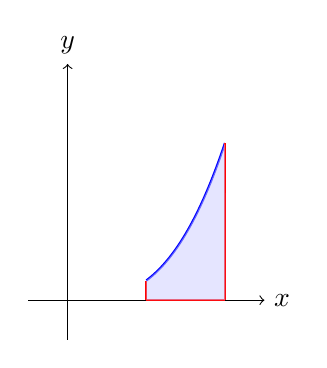
\begin{tikzpicture}[scale=1]
            % Axes
            \draw[->] (-0.5,0) -- (2.5,0) node[right] {$x$};
            \draw[->] (0,-0.5) -- (0,3) node[above] {$y$};
            
            % Curve: y = x^3 (scaled in y-direction)
            \draw[thick,blue] plot[domain=1:2,samples=100] (\x,{0.25*\x^3});
            
            % Lines x=1 and x=2
            \draw[thick,red] (1,0) -- (1,0.25) ;
            \draw[thick,red] (2,0) -- (2,2) ;
            
            % Line y=0
            \draw[thick,red] (1,0) -- (2,0);
            
            % Shaded region
            \fill[blue!20,opacity=0.5] 
                (1,0) -- plot[domain=1:2,samples=100] (\x,{0.25*\x^3}) -- (2,0) -- cycle;
        \end{tikzpicture}
    \end{center}
    The volume generated by rotating the region is:
    \[2\pi\int_1^2 x(x^3) dx = 2\pi\int_1^2 x^4 dx = 2\pi(\frac{x^5}{5})|_1^2 = 2\pi(\frac{2^5}{5} - \frac{1^5}{5}) = 2\pi(\frac{32}{5} - \frac{1}{5}) = \frac{62\pi}{5}\]

\setcounter{enumi}{11}
    \item Use the method of cylindrical shells to find the volume generated by rotating the region bounded by the given curves about the y-axis.
    \[y=x^2, 0\leq x \leq 2,y =4 ,x=0\]
    \begin{center}
        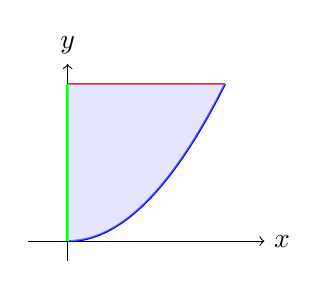
\begin{tikzpicture}[xscale=1,yscale=0.5] % Adjust scaling factors
            % Axes
            \draw[->] (-0.5,0) -- (2.5,0) node[right] {$x$};
            \draw[->] (0,-0.5) -- (0,4.5) node[above] {$y$};
            
            % Parabola y = x^2
            \draw[thick,blue,domain=0:2,samples=100] plot (\x,{(\x)^2});
            
            % Line y = 4
            \draw[thick,red] (0,4) -- (2,4);
            
            % Line x = 0
            \draw[thick,green] (0,0) -- (0,4);
            
            % Shaded area
            \fill[blue!20,opacity=0.5] (0,0) 
                -- plot[domain=0:2,samples=100] (\x,{(\x)^2}) 
                -- (2,4) 
                -- (0,4) -- cycle;
        \end{tikzpicture}
    \end{center}
    The volume generated by rotating the region is:
    \[2\pi\int_{0}^{2} x(x^2)dx = 2\pi\int_{0}^{2} (x^3)dx = 2\pi(\frac{x^4}{4})|_0^2 = 2\pi(\frac{2^4}{4}) = 8\pi\]
\newpage
\setcounter{enumi}{15}
    \item Use the method of cylindrical shells to find the volume of the solid obtained by rotating the region bounded by the given curves about the x-axis.
    \[y=\sqrt{x}, x = 0, y = 2\]
    \begin{center}
        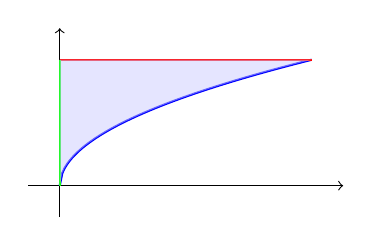
\begin{tikzpicture}[xscale=0.8,yscale=0.8] % Adjust scaling as needed
            % Axes
            \draw[->] (-0.5,0) -- (4.5,0);
            \draw[->] (0,-0.5) -- (0,2.5);
            
            % Curve y = sqrt(x)
            \draw[thick,blue,domain=0:4,samples=100] plot (\x,{sqrt(\x)});
            
            % Line y = 2
            \draw[thick,red] (0,2) -- (4,2);
            
            % Line x = 0
            \draw[thick,green] (0,0) -- (0,2);
            
            % Shaded area
            \fill[blue!20,opacity=0.5] (0,0) 
                -- plot[domain=0:4,samples=100] (\x,{sqrt(\x)}) 
                -- (4,2) 
                -- (0,2) -- cycle;
        \end{tikzpicture}
    \end{center}
    \[2 = \sqrt{x}\]
    \[x = 4\]
    The volume generated by rotating the region is:
    \[2\pi\int_0^4x(2-\sqrt{x})dx = 2\pi\int_0^4(2x-x\sqrt{x})dx = 2\pi(x^2 - \frac{2x^{5/2}}{5})|_0^4 \]
    \[= 2\pi(4^2 - \frac{2\times4^{5/2}}{5} - 2^2 + \frac{2\times2^{5/2}}{5}) = 2\pi(\frac{-4 + 2\sqrt{2^5}}{5})\]
\setcounter{enumi}{17}
    \item Use the method of cylindrical shells to find the volume of the solid obtained by rotating the region bounded by the given curves about the x-axis.
    \[x = -3y^2 + 12y - 9, x = 0\]
    \begin{center}
        \begin{tikzpicture}[xscale=0.5,yscale=0.5] % Adjust scaling as needed
            % Axes
            \draw[->] (-1,0) -- (4,0) node[right] {$x$};
            \draw[->] (0,0) -- (0,4) node[above] {$y$};
        
            % Curve x = -3y^2 + 12y - 9 (right side only)
            \draw[thick,blue,domain=1:3,samples=100] 
                plot ({-3*(\x)^2 + 12*(\x) - 9}, \x);
        \end{tikzpicture}
    \end{center}
    \[0 = -3y^2 + 12y- 9\]
    \[y = 1 \text{, or }y = 3\]
    The volume generated by rotating the region is:
    \[2\pi\int_1^3y(-3y^2 + 12y - 9)dy = 2\pi\int_1^3(-3y^3 + 12y^2 - 9y)dy = 2\pi(-\frac{3y^4}{4} + 4y^3 - \frac{9y^2}{2})|_1^3\]
    \[= 2\pi(-\frac{3\times3^4}{4} + 4\times3^3 - \frac{9\times3^2}{2} + \frac{3\times1^4}{4} - 4\times1^3 + \frac{9\times1^2}{2}) = 16\pi\]
\newpage
\setcounter{enumi}{23}  
    \item A solid is obtained by rotating the shaded region about the specified axis. 
    \begin{center}
        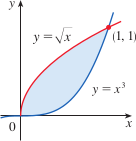
\includegraphics{img/img-0.png}\\
        About y = -1.
    \end{center}
    \begin{enumerate}
        \item Sketch the solid and a typical approximating cylindrical shell.
        \item Use the method of cylindrical shells to set up an integral for the volume of the solid.
        \[2\pi\int_0^1x(\sqrt{x} - x^3)dx\]
        \item Evaluate the integral to find the volume
        \[2\pi\int_0^1x(\sqrt{x} - x^3)dx = 2\pi\int_0^1(x\sqrt{x} - x^4)dx = 2\pi(\frac{2x^{5/2}}{5} - \frac{x^5}{5})|_0^1\]
        \[=2\pi(\frac{2\times1^{5/2}}{5} - \frac{1^5}{5}) = \frac{2\pi}{5}\]
    \end{enumerate}
\setcounter{enumi}{25}  
    \item Use the method of cylindrical shells to find the volume generated by rotating the region bounded by the given curves about the specified axis.
    \[y=4-2x,y=0,x=0\text{; about x = -1}\]
    \begin{center}
        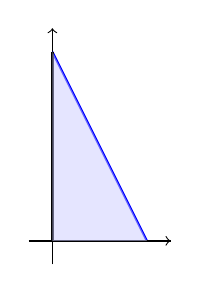
\begin{tikzpicture}[xscale=0.6,yscale=0.6] % Adjust scaling as needed
            % Axes
            \draw[->] (-0.5,0) -- (2.5,0);
            \draw[->] (0,-0.5) -- (0,4.5);
        
            % Line y = 4 - 2x
            \draw[thick,blue,domain=0:2] plot (\x,{4 - 2*\x});
            
            % Line y = 0 (x-axis)
            \draw[thick] (-0.5,0) -- (2.5,0);
            
            % Line x = 0 (y-axis)
            \draw[thick] (0,0) -- (0,4);
        
            % Shaded area
            \fill[blue!20,opacity=0.5] 
                (0,0) -- (0,4) -- (2,0) -- cycle;
        \end{tikzpicture}
    \end{center}
    \[0 = 4-2x\]
    \[x = 2\]
    The volume generated by rotating the region is:
    \[2\pi\int_0^2 (x+1)(4-2x)dx = 2\pi\int_0^2 (-2x^2+2x+4)dx = 2\pi(-\frac{2x^3}{3} + x^2 + 4x)|_0^2\]
    \[ = 2\pi(-\frac{2\times2^3}{3} + 2^2 + 4\times2) = 2\pi(-\frac{16}{3} + 12) = \frac{40\pi}{3}\]
\newpage
\setcounter{enumi}{35}
    \item Let:
    \[x^2-y^2=7,x=4\text{; about }y = 5\]
    \begin{center}
        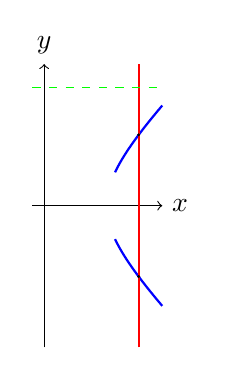
\begin{tikzpicture}[scale=0.3] % Adjust scaling as needed
            % Axes
            \draw[->] (-0.5,0) -- (5,0) node[right] {$x$};
            \draw[->] (0,-6) -- (0,6) node[above] {$y$};
        
            % Right branch of hyperbola x^2 - y^2 = 7 (x >= 0)
            \draw[thick,blue,domain=3:5,samples=1000] plot (\x,{sqrt((\x)^2 - 7)});
            \draw[thick,blue,domain=3:5,samples=1000] plot (\x,{-sqrt((\x)^2 - 7)});
        
            % Line x = 4
            \draw[thick,red] (4,-6) -- (4,6);
        
            % Highlight area around y = 5
            \draw[dashed,green] (-0.5,5) -- (5,5);
        
            % Add intersection points for emphasis
            \fill[black] (4,{sqrt(16 - 7)}) circle (2pt);
            \fill[black] (4,{-sqrt(16 - 7)}) circle (2pt);
        \end{tikzpicture}
    \end{center}
    \begin{enumerate}
        \item Set up an integral for the volume of the solid obtained by rotating the region bounded by the given curve about the specified axis.
        \[x^2-y^2 = 7\]
        \[x^2 = y^2 + 7\]
        \[x = \sqrt{y^2 + 7}\]
        Let x = 4:
        \[y^2 = 4^2 - 7 = 9\]
        \[y = \pm 3\]
        \[2\pi\int_{-3}^{3} (5-y)(4-\sqrt{y^2+7})dy\]
        \item Use a calculator or computer to evaluate the integral correct to five decimal places.
        \[2\pi\int_{-3}^{3} (5-y)(4-\sqrt{y^2+7})dy \approx 163.02712\]
    \end{enumerate}
\end{enumerate}

Section 5.4:

\begin{enumerate}
    \item How much work is done when a weight lifter lifts 200 kg from 1.5m to 2m above the ground?
    \[F = 200\times9.8 = 1960\]
    \[W = 1960 \times (2-1.5) = 980J\]
\setcounter{enumi}{2}
    \item A variable force of $5x^{-2}$ pounds moves an object along a straight line when it is $x$ feet from the origin. Calculate the work done in moving the object from $x=1$ ft to $x=10$ ft.
    \[\int_{1}^{10}5x^{-2}dx = 4.5\text{ft-lb}\]
\setcounter{enumi}{6}
    \item A force of 10lb is required to hold a spring stretched 4in. beyond its natural length. How much work is done in stretching it from its natural length to 6in. beyond its natural length?
    \[kx = 10\]
    \[4k = 10\]
    \[k = \frac{5}{2}\]
    \[W = \int_0^6 \frac{5}{2}x = (\frac{5}{2}\frac{x^2}{2})|_0^6 = (\frac{5}{2}\frac{6^2}{2}) = 45\text{ft-lb}\]
    \item A spring has a natural length of 40cm. If a 60-N force is required to keep the spring compressed 10cm, how much work is done during this compression? How much work is required to compress the spring to a length of 25cm?
    \[kx = 60\]
    \[k0.1 = 60\]
    \[k = 600\]
    \[W_1 = \int_{0}^{0.1}600x = (300x^2)|^{0.1}_0 = 3(J)\]
    \[W_2 = \int_{0}^{0.15}600x = (300x^2)|^{0.15}_0 = 6.75(J)\]

\setcounter{enumi}{16}
    \item A 10-ft chain weighs 25 lb and hangs from a ceiling. Find the work done in lifting the lower end of the chain to the ceiling so that it is level with the upper end.
    \[\text{weight per ft} = \frac{25}{10} = 2.5\]
    \[W = \int_{0}^{10} 2.5x dx = 2.5(\frac{x^2}{2})|_0^{10} = 2.5(\frac{10^2}{2}) = 125\text{(ft-lb)}\]

\setcounter{enumi}{19}
    \item A circular swimming pool has a diameter of 24ft, the sides are 5ft high, and the depth of the water is 4ft. How much work is required to pump all of the water out over the side? (Use the fact that water weighs $62.5lb/ft^3$.)
    \[W = \int_{0}^{4}(5-y)12^2\times\pi\times62.5 = 108000\pi\]

\setcounter{enumi}{22}
    \item A tank is full of water. Find the work required to pump the water out of the spout. 
    \begin{center}
        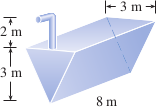
\includegraphics{img/img-1.png}
    \end{center}
    The triangle function is:
    \[f(x) = 2x = y\]
    \[x = \frac{y}{2}\]
    \[W = 9800\int_{0}^{3}(5-y) \times (\frac{y}{2})\times 2 \times 8dy = 1058400(J)\]
\end{enumerate}

Section 5.5:

\begin{enumerate}
    \item Find the average value of the function on the given interval.
    \[f(x) = 3x^2 + 8x, [-1,2]\]
    The average value of the function on the given inteval is:
    \[f_{avg} = \frac{1}{2-(-1)}\int_{-1}^2 3x^2 + 8x dx = \frac{1}{3}\int_{-1}^2 3x^2 + 8x dx = 7\]

\setcounter{enumi}{2}
    \item Find the average value of the function on the given interval.
    \[g(x) = 3\cos x ,[-\frac{\pi}{2},\frac{\pi}{2}] \]
    The average value of the function on the given inteval is:
    \[f_{avg} = \frac{1}{\pi}\int_{-\pi/2}^{\pi/2} 3\cos x dx = \frac{1}{\pi}(3\sin x)|_{-\pi/2}^{\pi/2} = \frac{6}{\pi}\]

\setcounter{enumi}{8}
    \item Let:
    \[f(t) = \frac{1}{t^2}, [1,3]\]
    \begin{enumerate}
        \item Find the average value of $f$ on the given interval.
        \[f_{avg} = \frac{1}{3-1}\int_1^3 \frac{1}{t^2} dt = \frac{1}{2}\int_1^3 \frac{1}{t^2} dt = \frac{1}{2}(-\frac{1}{t})|_{1}^{3} = \frac{1}{3}\]
        \item Find $c$ in the given interval such that $f_{avg} = f(c)$.
        \[f(c) = \frac{1}{3}\]
        \[\frac{1}{c^2} = \frac{1}{3}\]
        \[c^2 = \frac{1}{3}\]
        \[c = \pm \sqrt{\frac{1}{3}}\]
        Because $c$ is in the interval $[1,3]$.
        \[c = \sqrt{\frac{1}{3}}\]
        \item Sketch the graph of $f$ and a rectangle whose base is the given interval and whose area is the same as the area under the graph of $f$.
    \end{enumerate}
    \begin{center}
        \begin{tikzpicture}[scale=0.8]
            \begin{axis}[
                axis lines=middle,
                xlabel={$t$},
                ylabel={$f(t)$},
                xmin=0, xmax=4,
                ymin=0, ymax=2,
                domain=1:3,
                samples=100,
                legend style={at={(1,1)}, anchor=north east}
            ]
                % Plot the function
                \addplot[blue, thick] {1/(x^2)};
                \addlegendentry{$f(t) = \frac{1}{t^2}$}
            \end{axis}
        \end{tikzpicture}
    \end{center}

\setcounter{enumi}{14}  
    \item Find the average value of $f$ on [0,8].
    \begin{center}
        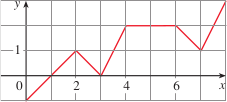
\includegraphics{img/img-2.png}
    \end{center}
    The average value of $f$ on [0,8] is the area under $f$ divided by the range of the interval.
    \[f_{avg} = \frac{9}{8}\]

\setcounter{enumi}{18}
    \item The linear density in a rod 8m long is $12/\sqrt{x+1} \text{ kg/m}$, where $x$ is measured in meters from one end of the rod. Find the average density of the rod.
    \[\text{The average density of the rod} = \frac{1}{8} \int_0^8 \frac{12}{\sqrt{x+1}}dx = 6\text{kg/m}\]


\end{enumerate}

\end{document}